To evaluate the performance of the proposed control scheme, we apply it to an idealized tracking and navigation problem in a 2-dimensional plane.
The estimator, which is an anytime algorithm, is responsible for localization of a vehicle. % in the 2-d space.
The controller, which is the RMPC algorithm, is tasked with moving the vehicle to the origin while keeping it inside a safe set.
The continuous-time state-space representation of the vehicle is
\begin{equation*}
\begin{bmatrix} \dot{x} \\ \dot{y} \\ \dot{v_x} \\ \dot{v_y} \end{bmatrix} = \begin{bmatrix} 0&0&1&0 \\ 0&0&0&1 \\0&0&0&0 \\0&0&0&0  \end{bmatrix}
\begin{bmatrix} x \\ y \\ v_x \\ v_y \end{bmatrix} +
\begin{bmatrix} 0&0 \\ 0&0 \\ 1&0 \\ 0&1 \end{bmatrix}
\begin{bmatrix} a_x \\ a_y \end{bmatrix} \text.
\end{equation*}
%\begin{subequations}
% \begin{align}
% \begin{bmatrix} \dot{x} \\ \dot{y} \\ \dot{v_x} \\ \dot{v_y} \end{bmatrix} &= A \begin{bmatrix} x \\ y \\ v_x \\ v_y \end{bmatrix} + B \begin{bmatrix} a_x \\ a_y \end{bmatrix} \\
% A&= \begin{bmatrix} 0&0&1&0 \\ 0&0&0&1 \\0&0&0&0 \\0&0&0&0  \end{bmatrix} \text{ , }
% B= \begin{bmatrix} 0&0 \\ 0&0 \\ 1&0 \\ 0&1 \end{bmatrix}
% \end{align}
%\end{subequations}
%
Here, the states are position along x-axis ($x$), position along y-axis ($y$), velocity along x-axis ($v_x$), and velocity along y-axis ($v_y$).
The control inputs are acceleration along x-axis ($a_x$) and acceleration along y-axis ($a_y$).
The sampling period for discrete-time implementation of the controller and the estimator is $T=0.02s$.
For simplicity, we assume that there is no process noise.


\subsection{The state estimator}
In this study, we assume that the estimator is a vision-based system which can give estimates of the 4 states.
For example, the estimator can utilize a camera looking down on the vehicle in the $x$--$y$ plane, and the captured images are processed to detect and localize the vehicle as well as to estimate its velocity.
There are three estimation modes $\left(\sDelay[1]=10\mathrm{ms}, \sAccu[1]=0.1\right)$, $\left(\sDelay[2]=5\mathrm{ms}, \sAccu[2]=0.5\right)$, $\left(\sDelay[3]=2.5\mathrm{ms}, \sAccu[3]=1.0\right)$, assuming a linear relation between computation time and estimation accuracy.
The realization of these modes can come from the use of different camera resolutions, frame rates as well as feature tracking/estimation algorithms, which is beyond the scope of this paper.
The estimation error is such that $\norm{e_{k}}_\infty \leq \sAccu[k]$ where $e_{k}= x_{k}-\hat{x}_{k}$.
In our simulation, the state estimate $\hat{x}_{k}$ is generated by adding a uniformly random error $e_{k}$, bounded by $\sAccu[k]$, to the true state $x_{k}$.
%The error is chosen to be within the upper bounds of the estimation error for the estimation mode. 

\subsection{Simulation setup and results}

%Given the three estimation modes, the plant model and the state and input constraints, 
The controller is tasked with minimizing a $\ell_2$-norm cost on the states and inputs while respecting the state and input constraints.
When the origin is within the safe set of positions, this minimization results in a trajectory bringing the vehicle from an initial displacement to the origin.
We chose %a sampling time of $T=0.02s$, ==> redundant
a horizon length $N = 50$ for the RMPC and a simulation length of 400 time steps.
For the scope of this study, we neglected the cost of using a particular estimation mode, \ie $\alpha=0$ in \algoref{RMPC-algo}.
This means that the mode selection depends solely on the control performance for the RMPC formulation for that mode. Note, the computations for the feasible set were done using the results of \secref{ComputePontryagin}, which gave a significant speed up. Discrete time LQR design was used to select %come up with
a time-invariant stabilizing feedback gain $K(\sDelay)$ for each estimation mode.% compared to existing toolboxes. %This also enabled us to use \algoref{RMPC-algo-improved}, which we did not implement as we had only 3 modes, but is straightforward to implement if we have many modes. 
The robust control invariant set $\CCC(\sDelay, \sAccu)$ was computed using the Matlab invariant set toolbox \cite{invset}.
The RMPC optimization was solved in MATLAB using CVX \cite{cvx}, \cite{cvx2}.

For the simulation, the initial state was set to be $\left[30,30,0,0\right]$ corresponding to initial position of $30,30$ units in the x--y plane and zero initial velocities (in both directions). The initial inputs were also set to zero. \figref{TrackingTrajectory_scissored} shows the estimated trajectory and the actual trajectory of the system, which stays inside the safe set of positions (the polyhedron in the figure). The velocities were constrained such that $\|v_{x}(t)\|_\infty \leq 100, \forall t$ and $\|v_{y}(t)\|_\infty \leq 100, \forall t$. The inputs were also constrained to be such that $\|a_x(t)\|_\infty \leq 100, \forall t$ and $\|a_y(t)\|_\infty \leq 10, \forall t$. The initial feasible set $\ZSet$ can be found by the Cartesian product of these three (the position, velocity and acceleration) sets. Initially, the estimator was started in the 1$^{st}$ mode. Using \algoref{RMPC-algo}, the optimal mode of the estimator and the corresponding Robust MPC input to the system are picked at each time step. Note that the actual trajectory is nearly a straight line from the initial point to the origin, as it would be in a noiseless and delay free system, even though the measured trajectory shows the effects of the estimation error and computation delay. This shows the robustness of the RMPC algorithm in the presence of time varying delays and estimation errors due the estimator mode switching. \figref{velocities} shows the velocities (both estimated and actual). Note that as expected, the vehicle slows down as it approaches the origin and the trend continues even as estimation error increases. \figref{inputs} shows the acceleration inputs to the system. Note, the main assumption behind this work is that there is a benefit from switching between different ($\sDelay, \sAccu$) estimation modes. \figref{modes} shows the mode selected at each time step and the switching of the modes indicates that there is indeed a cost improvement in switching modes while maintaining feasibility. This shows \algoref{RMPC-algo} gives better performance than a Robust MPC formulation with a fixed delay/estimation error mode.

\begin{figure}
  \centering
  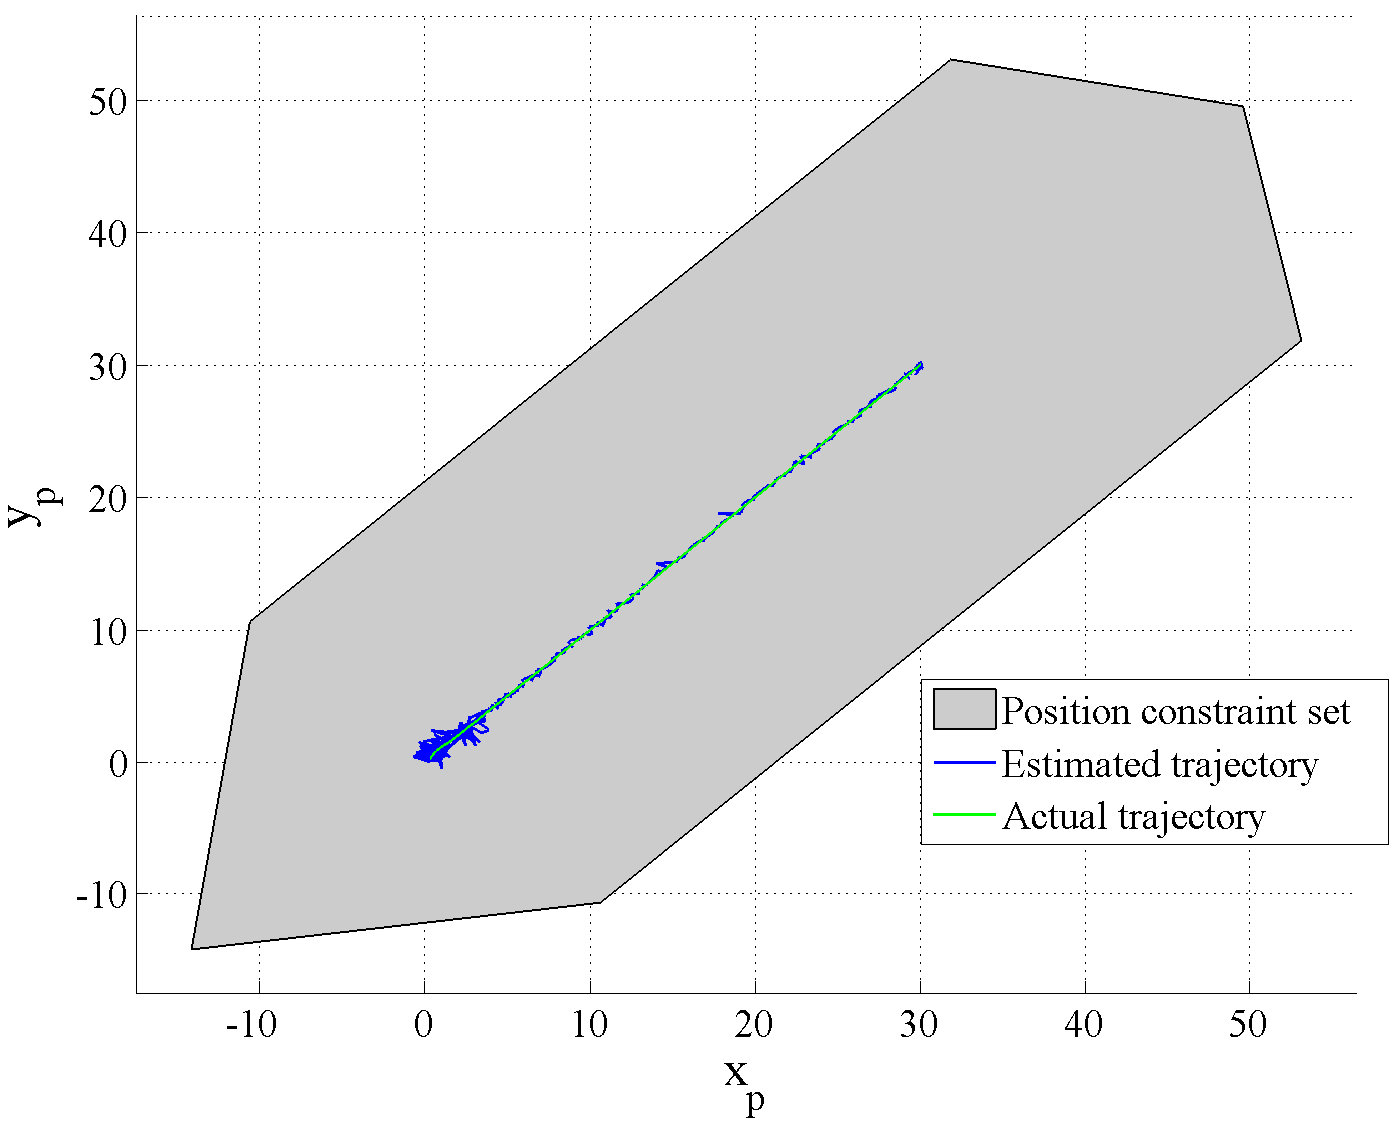
\includegraphics[width=0.8\columnwidth]{figs/TrackingTrajectory_scissored.pdf}
  \caption{Trajectory and safe set of positions.}
  \label{fig:TrackingTrajectory_scissored}
\end{figure}

\begin{figure}
  \centering
  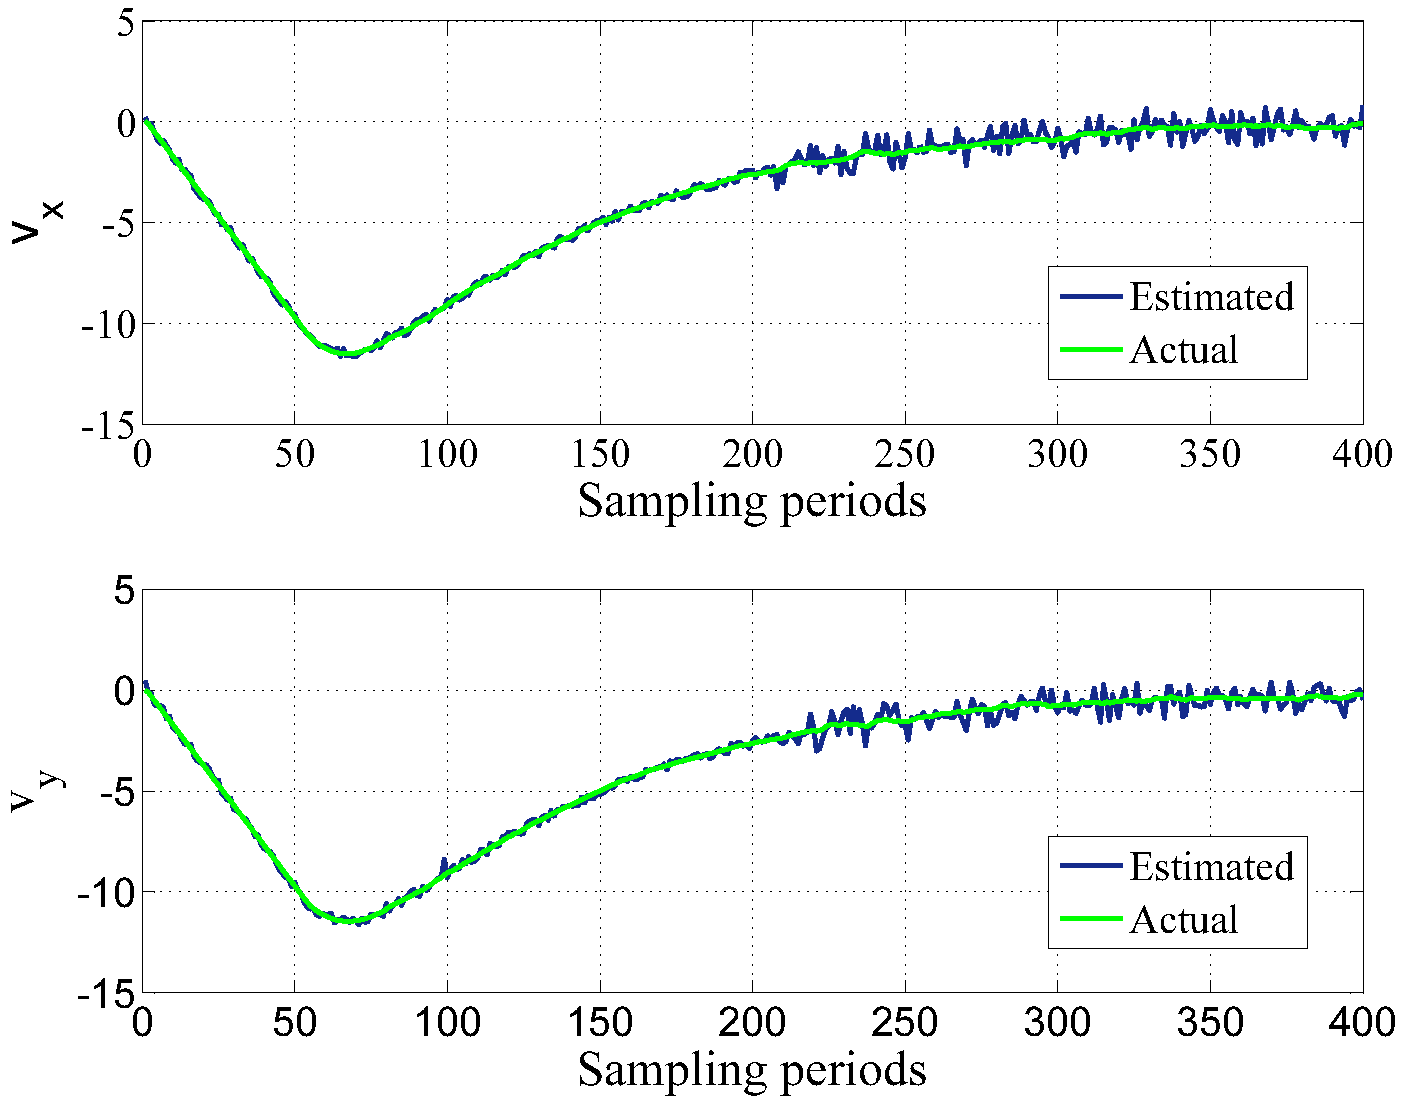
\includegraphics[width=0.80\columnwidth]{figs/velocities_scissored.pdf}
  \caption{Estimated and actual velocities of the vehicle.}
  \label{fig:velocities}
\end{figure}

\begin{figure}
  \centering
  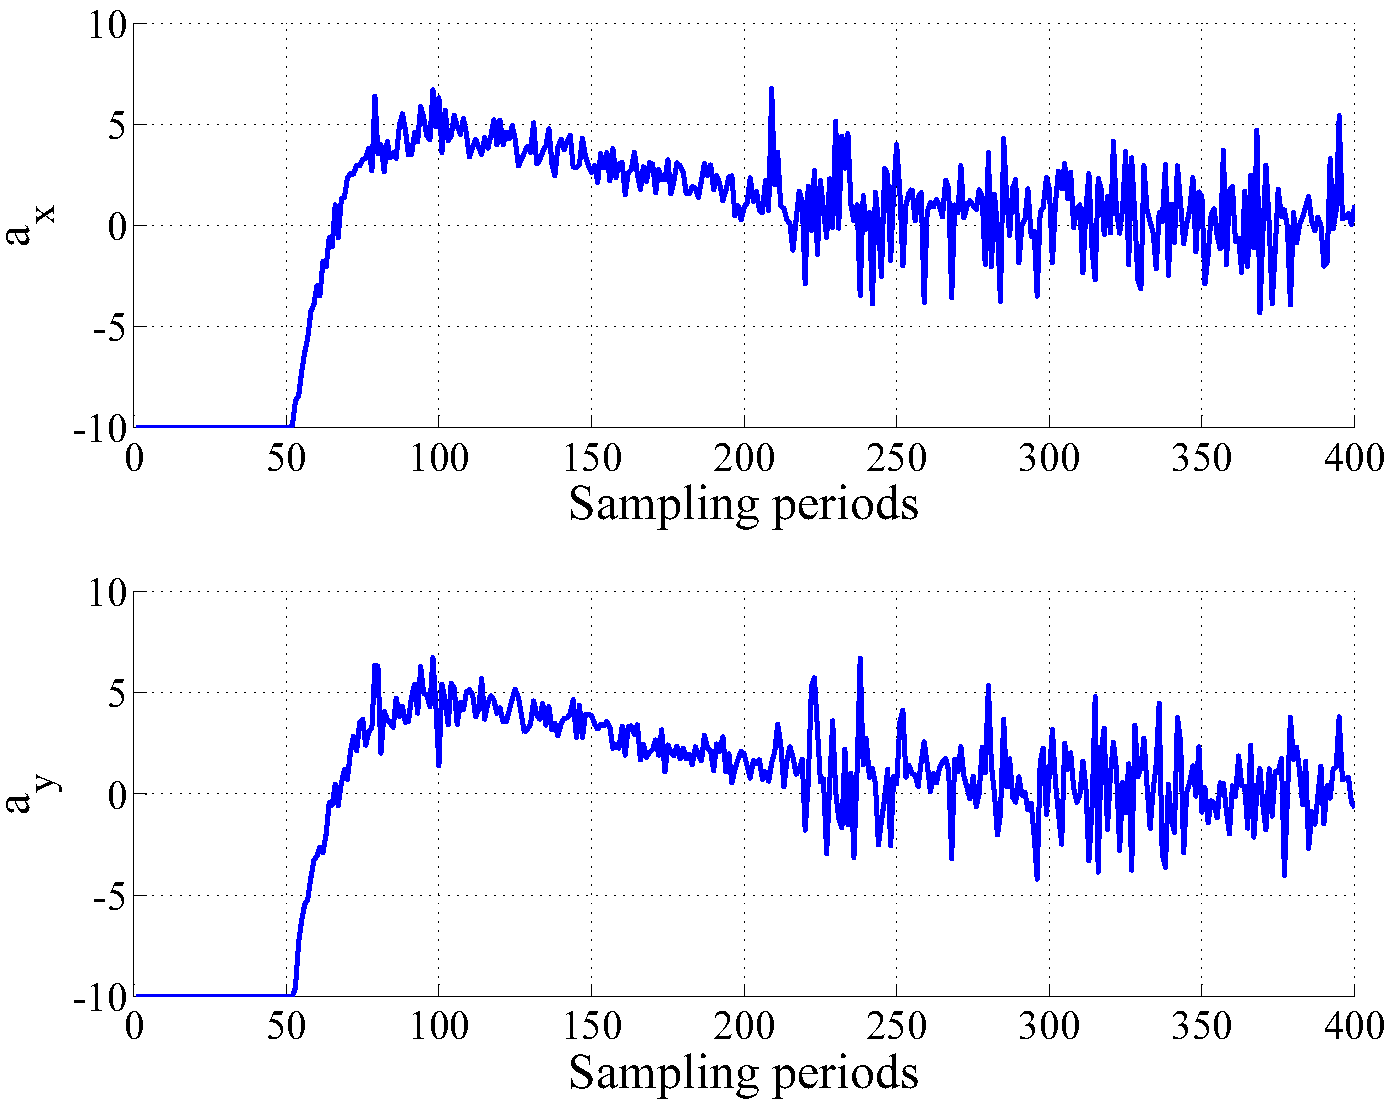
\includegraphics[width=0.80\columnwidth]{figs/inputs_scissored.pdf}
  \caption{Control input (acceleration) to the vehicle.}
  \label{fig:inputs}
\end{figure}

\begin{figure}
  \centering
  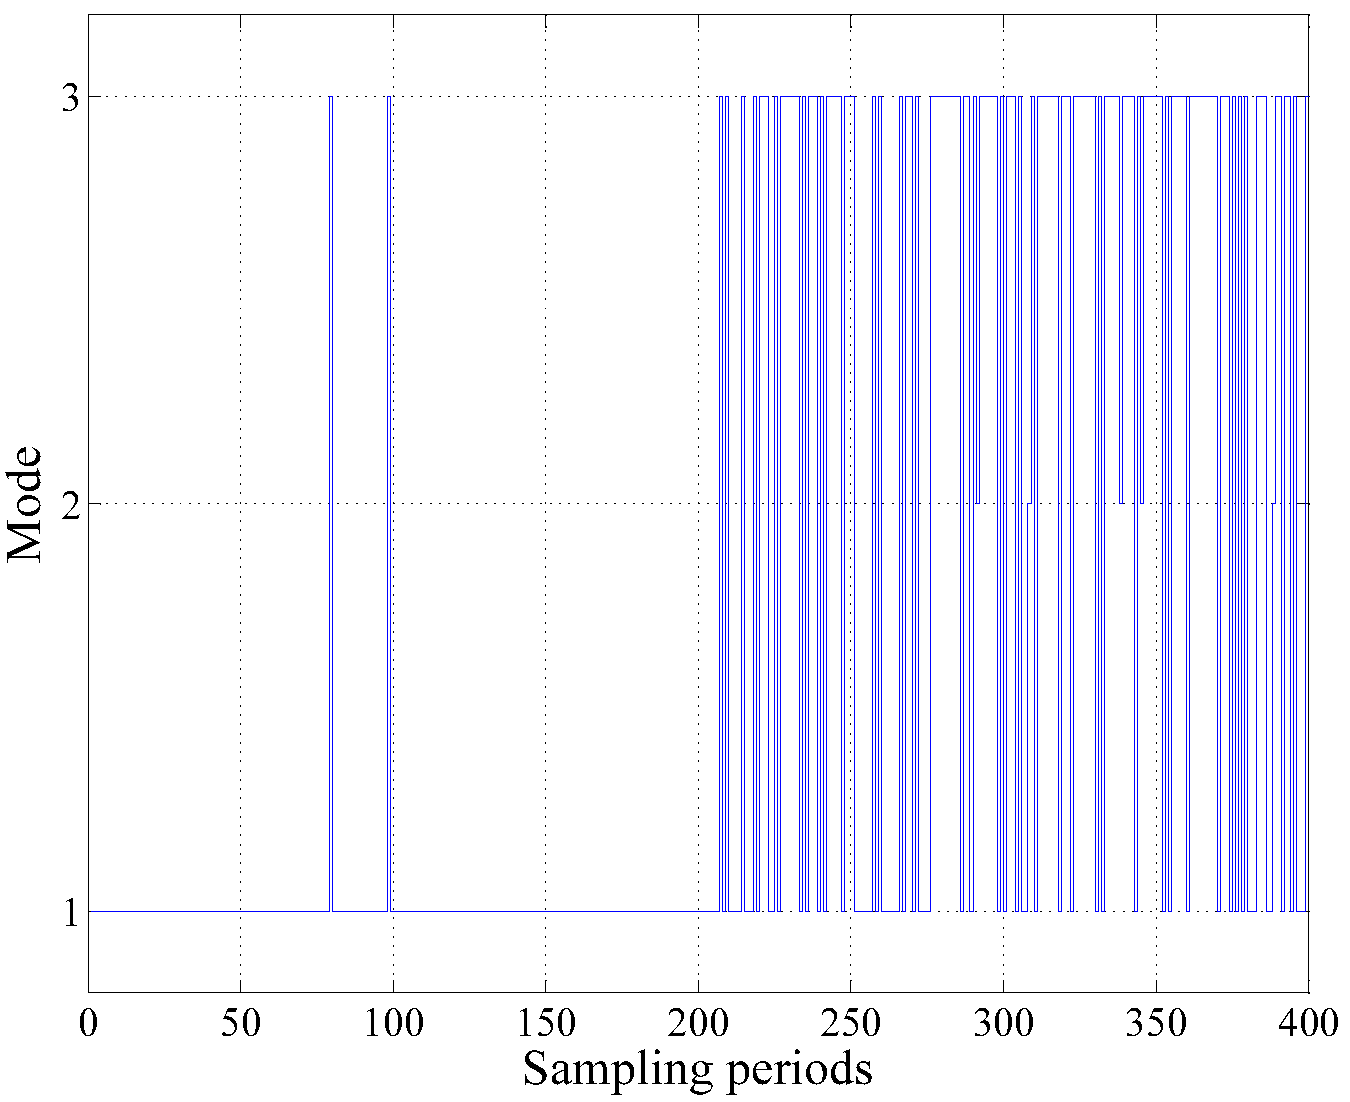
\includegraphics[width=0.9\columnwidth, height=38mm]{figs/ModePicked_scissored.pdf}
  \caption{Estimation mode switching of the proposed control algorithm.}
  \label{fig:modes}
\end{figure}


%%% Local Variables: 
%%% mode: latex
%%% TeX-master: "CDC14_Anytime_Main"
%%% End: 
